\documentclass[a4paper,11pt]{article}
\usepackage[left=2.5cm, right=2.5cm, top=1.5cm, bottom=1.5cm]{geometry}
\usepackage{graphicx}
\usepackage{amssymb}
\usepackage{amsmath}
\usepackage{xcolor}
\usepackage[active,tightpage]{preview}
\usepackage{hyperref}
\usepackage{pythonhighlight}

\hypersetup{ %color attributes of citation, link, etc.
    colorlinks=true,
    linkcolor=blue,
    filecolor=gray,
    urlcolor=blue,
    citecolor=blue,
}

\setlength{\parindent}{0pt}

\renewcommand{\PreviewBorder}{1in}
\newcommand{\Newpage}{\end{preview}\begin{preview}}
\newcommand{\matlab}{\textsc{Matlab}} %very important and totally necessary addition
\newcommand{\parallelsum}{\mathbin{\!/\mkern-5mu/\!}}

\newcommand\Item[1][]{%
  \ifx\relax#1\relax  \item \else \item[#1] \fi
  \abovedisplayskip=0pt\abovedisplayshortskip=0pt~\vspace*{-\baselineskip}}

%'codify' text for snippets
\usepackage{xcolor}
\definecolor{codegray}{gray}{1}
\newcommand{\code}[1]{\colorbox{codegray}{\texttt{#1}}}


\graphicspath{ {../images/} }
           
\begin{document}
\begin{preview}
\title{\LARGE{\textbf{ECEN405 Lab 1 Report\\Pulse Width Modulation}}}
\author{Niels Clayton : 300437590\\\textbf{Lab Partner:} Nickolai Wolfe}
\date{}
\maketitle
\hrule

\begin{enumerate}
    \item 
    $C_1 = 10\;nF$\\
    
    \item 
    $f_{min} = 297$ Hz\\$f_{max} = 3.03$ MHz\\
    
    \item 
    Schematic of the PWM generator
    \begin{center}
        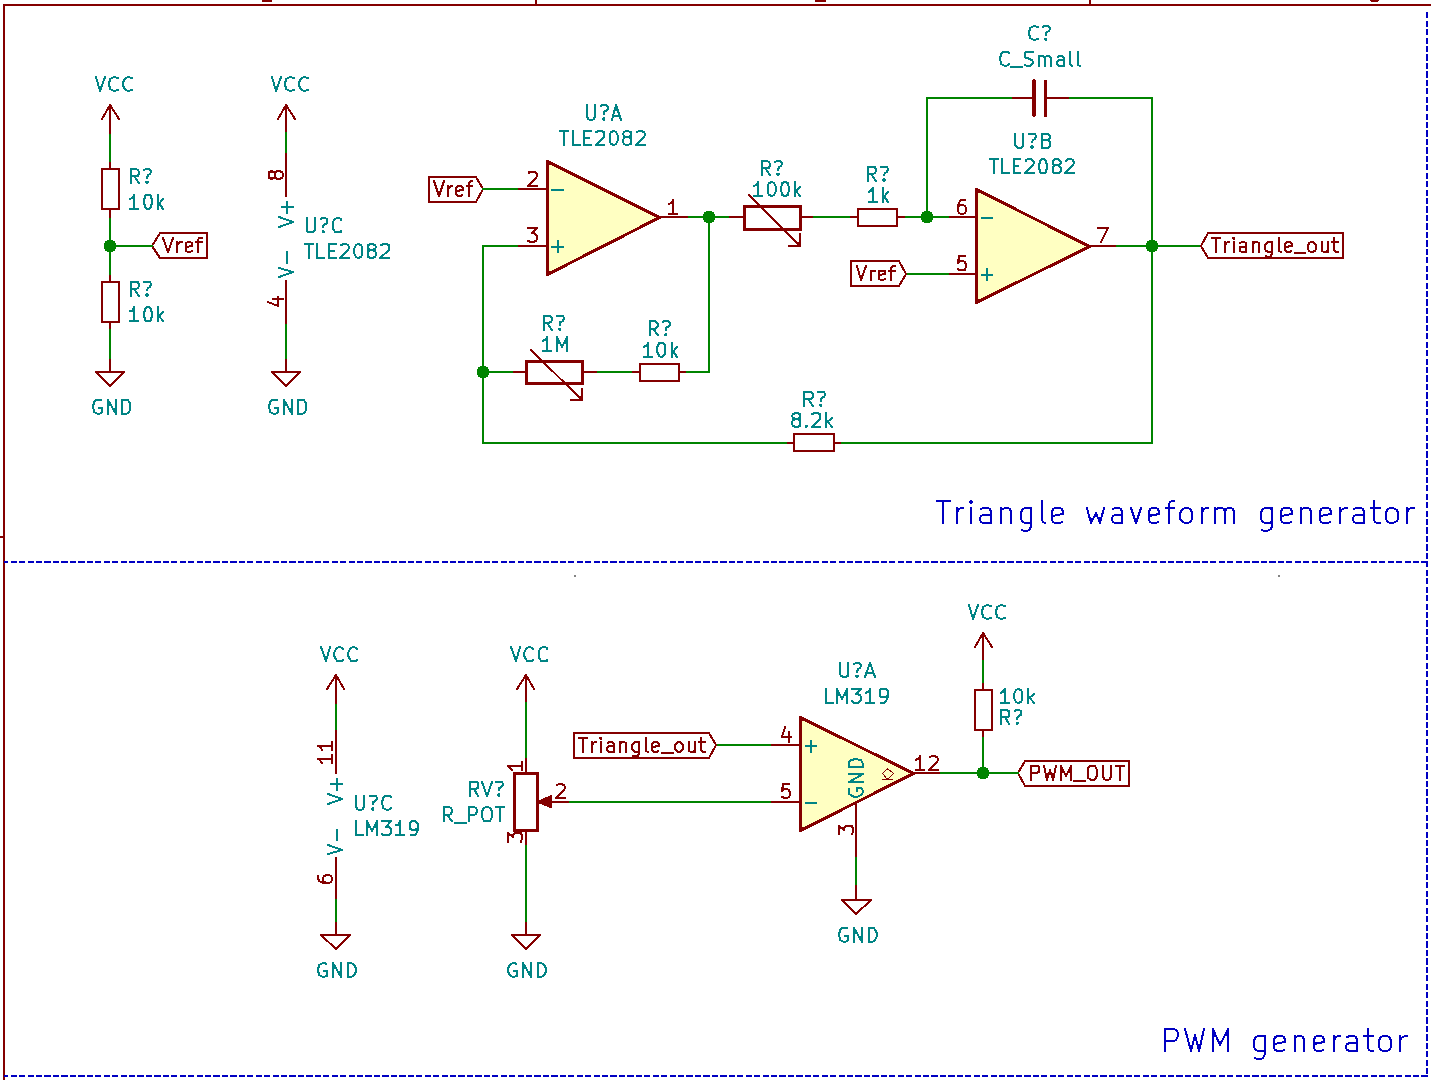
\includegraphics[width = \textwidth]{schematic_1.png}
    \end{center}
    \vspace{20pt}

    \item 
    Conduction losses: $$P_{cond} = 0.6\;W $$
    Minimum frequency switching losses $$P_{sw}= 78.4 \;\mu W$$
    Maximum frequency switching losses $$P_{sw}= 0.799 \; W$$\\
    
    \item 
    Actual photo capturing the look of approval on Danny B's face as I complete the circuit and proudly show him.
    \begin{center}
        
\includegraphics[width = \textwidth]{Danny_B.jpg}
    \end{center}
    \vspace{20pt}

    \item PUT PHOTOS HERE \\
    
    
    \item It was noted that the theoretical minimum and maximum achieved switching frequencies of the circuit were not achieved by the designed circuit. Although it is hard to exactly pinpoint where this issue comes from, there are a range of possible factors that would affect these frequencies. By creating the circuit on a breadboard, we introduce parasitic capacitances, and inductances to the circuit, which will affect the op-amps. It is also possible that op-amp characteristics such as slew rate are affecting the frequency of the output. \\
    
    
    \item To get both an inverted and non-inverted signal, you can switch the input terminals of the comparator. Since the LM319 is a dual comparator, it is possible to have both the inverted and non-inverted signals out from the same IC. \\
    

    \item INSERT BLOCK DIAGRAM


\end{enumerate}

\section*{Appendix}

\textbf{Q1:} Equation to calculate the capacitor size
$$ C_{1}=\frac{R_{2}+R_{3}}{4R_{1}\left(R_{4}+R_{5}\right)F_{T}} $$\\

\textbf{Q2:} Equations to calculate the minimum and maximum frequencies
$$ f_{min}=\frac{R_{2}}{4R_{1}\left(R_{4}+R_{5}\right)C_{1}} = 297\;Hz $$ \\
$$ f_{max}=\frac{R_{2}+R_{3}}{4R_{1}\cdot R_{5}\cdot C_{1}} = 3.03\;MHz $$\\

\textbf{Q4:} \\\\
Conduction switching losses:
$$ P_{cond} = R_{DS(on)} \cdot d \cdot I^2 = 0.6\;W $$
Minimum frequency switching losses:
$$ P_{sw} = \frac{1}{2}V_{in} \cdot I_o (t_{c(on)} + t_{c(off)})f_{min} = 78.4 \;\mu W $$
Maximum frequency switching losses:
$$ P_{sw} = \frac{1}{2}V_{in} \cdot I_o (t_{c(on)} + t_{c(off)})f_{max} = 0.799 \; W $$


\end{preview}
\end{document}